\documentclass[tikz,border=0pt]{standalone}
\pdfminorversion=7
\usepackage[T1]{fontenc}
\usepackage{lmodern,amsmath,amssymb,graphicx}
\usepackage{pgfplots}
\usetikzlibrary{arrows.meta,calc,positioning,patterns,decorations.pathreplacing}
\pgfplotsset{compat=1.18}
\definecolor{family}{RGB}{0,140,18}
\definecolor{familypale}{RGB}{225,255,226}
\definecolor{frozen}{RGB}{49,57,208}
\definecolor{frozenpale}{RGB}{234,235,255}
\definecolor{adapter}{RGB}{219,102,0}
\definecolor{adapterpale}{RGB}{255,196,135}
\definecolor{outputcol}{RGB}{120,38,130}
\definecolor{ink}{RGB}{33,33,33}
\definecolor{muted}{RGB}{105,105,105}
\tikzset{
 figure/.style={x=1pt,y=1pt,line cap=round,line join=round,text=ink,
   >={Stealth[length=7pt,width=6pt]},font=\fontsize{20}{24}\selectfont},
 title/.style={font=\fontsize{29}{33}\selectfont},
 heading/.style={font=\fontsize{22}{26}\selectfont},
 labeltext/.style={font=\fontsize{18}{22}\selectfont,align=center},
 smalllabel/.style={font=\fontsize{15}{19}\selectfont,align=center},
 equation/.style={font=\fontsize{24}{29}\selectfont,align=center},
 flow/.style={->,line width=1.3pt},
 fineflow/.style={->,line width=.8pt},
 target/.style={circle,fill=family,draw=white,line width=1.2pt,inner sep=0pt,minimum size=12pt},
 candidate/.style={circle,fill=white,draw=muted,line width=1.3pt,inner sep=0pt,minimum size=10pt},
 neuron/.style={circle,draw=frozen,fill=frozen!18,minimum size=13pt,inner sep=0pt,line width=.8pt}
}
\DeclareMathOperator{\rank}{rank}
\DeclareMathOperator{\row}{row}
\DeclareMathOperator{\col}{col}
\newcommand{\R}{\mathbb R}
\graphicspath{{assets/}}
\newcommand{\canvas}[1]{\path[use as bounding box] (0,0) rectangle (960,600);
  \node[title,anchor=west] at (36,557) {#1};}
\newcommand{\glyphgrid}[2]{
 \begin{scope}[shift={(#1,#2)}]
  \fill[white] (0,0) rectangle (136,136);
  \foreach \x/\y/\c in {1/1/80,2/2/80,2/3/45,3/4/45,3/5/45,4/5/100,4/6/45,5/6/45,5/4/45,5/2/100,6/1/80}{
    \fill[frozen!\c] (\x*17,\y*17) rectangle ++(17,17);
  }
  \draw[step=17pt,black!30,line width=.35pt] (0,0) grid (136,136);
  \draw[black!45,line width=.6pt] (0,0) rectangle (136,136);
 \end{scope}}

\begin{document}
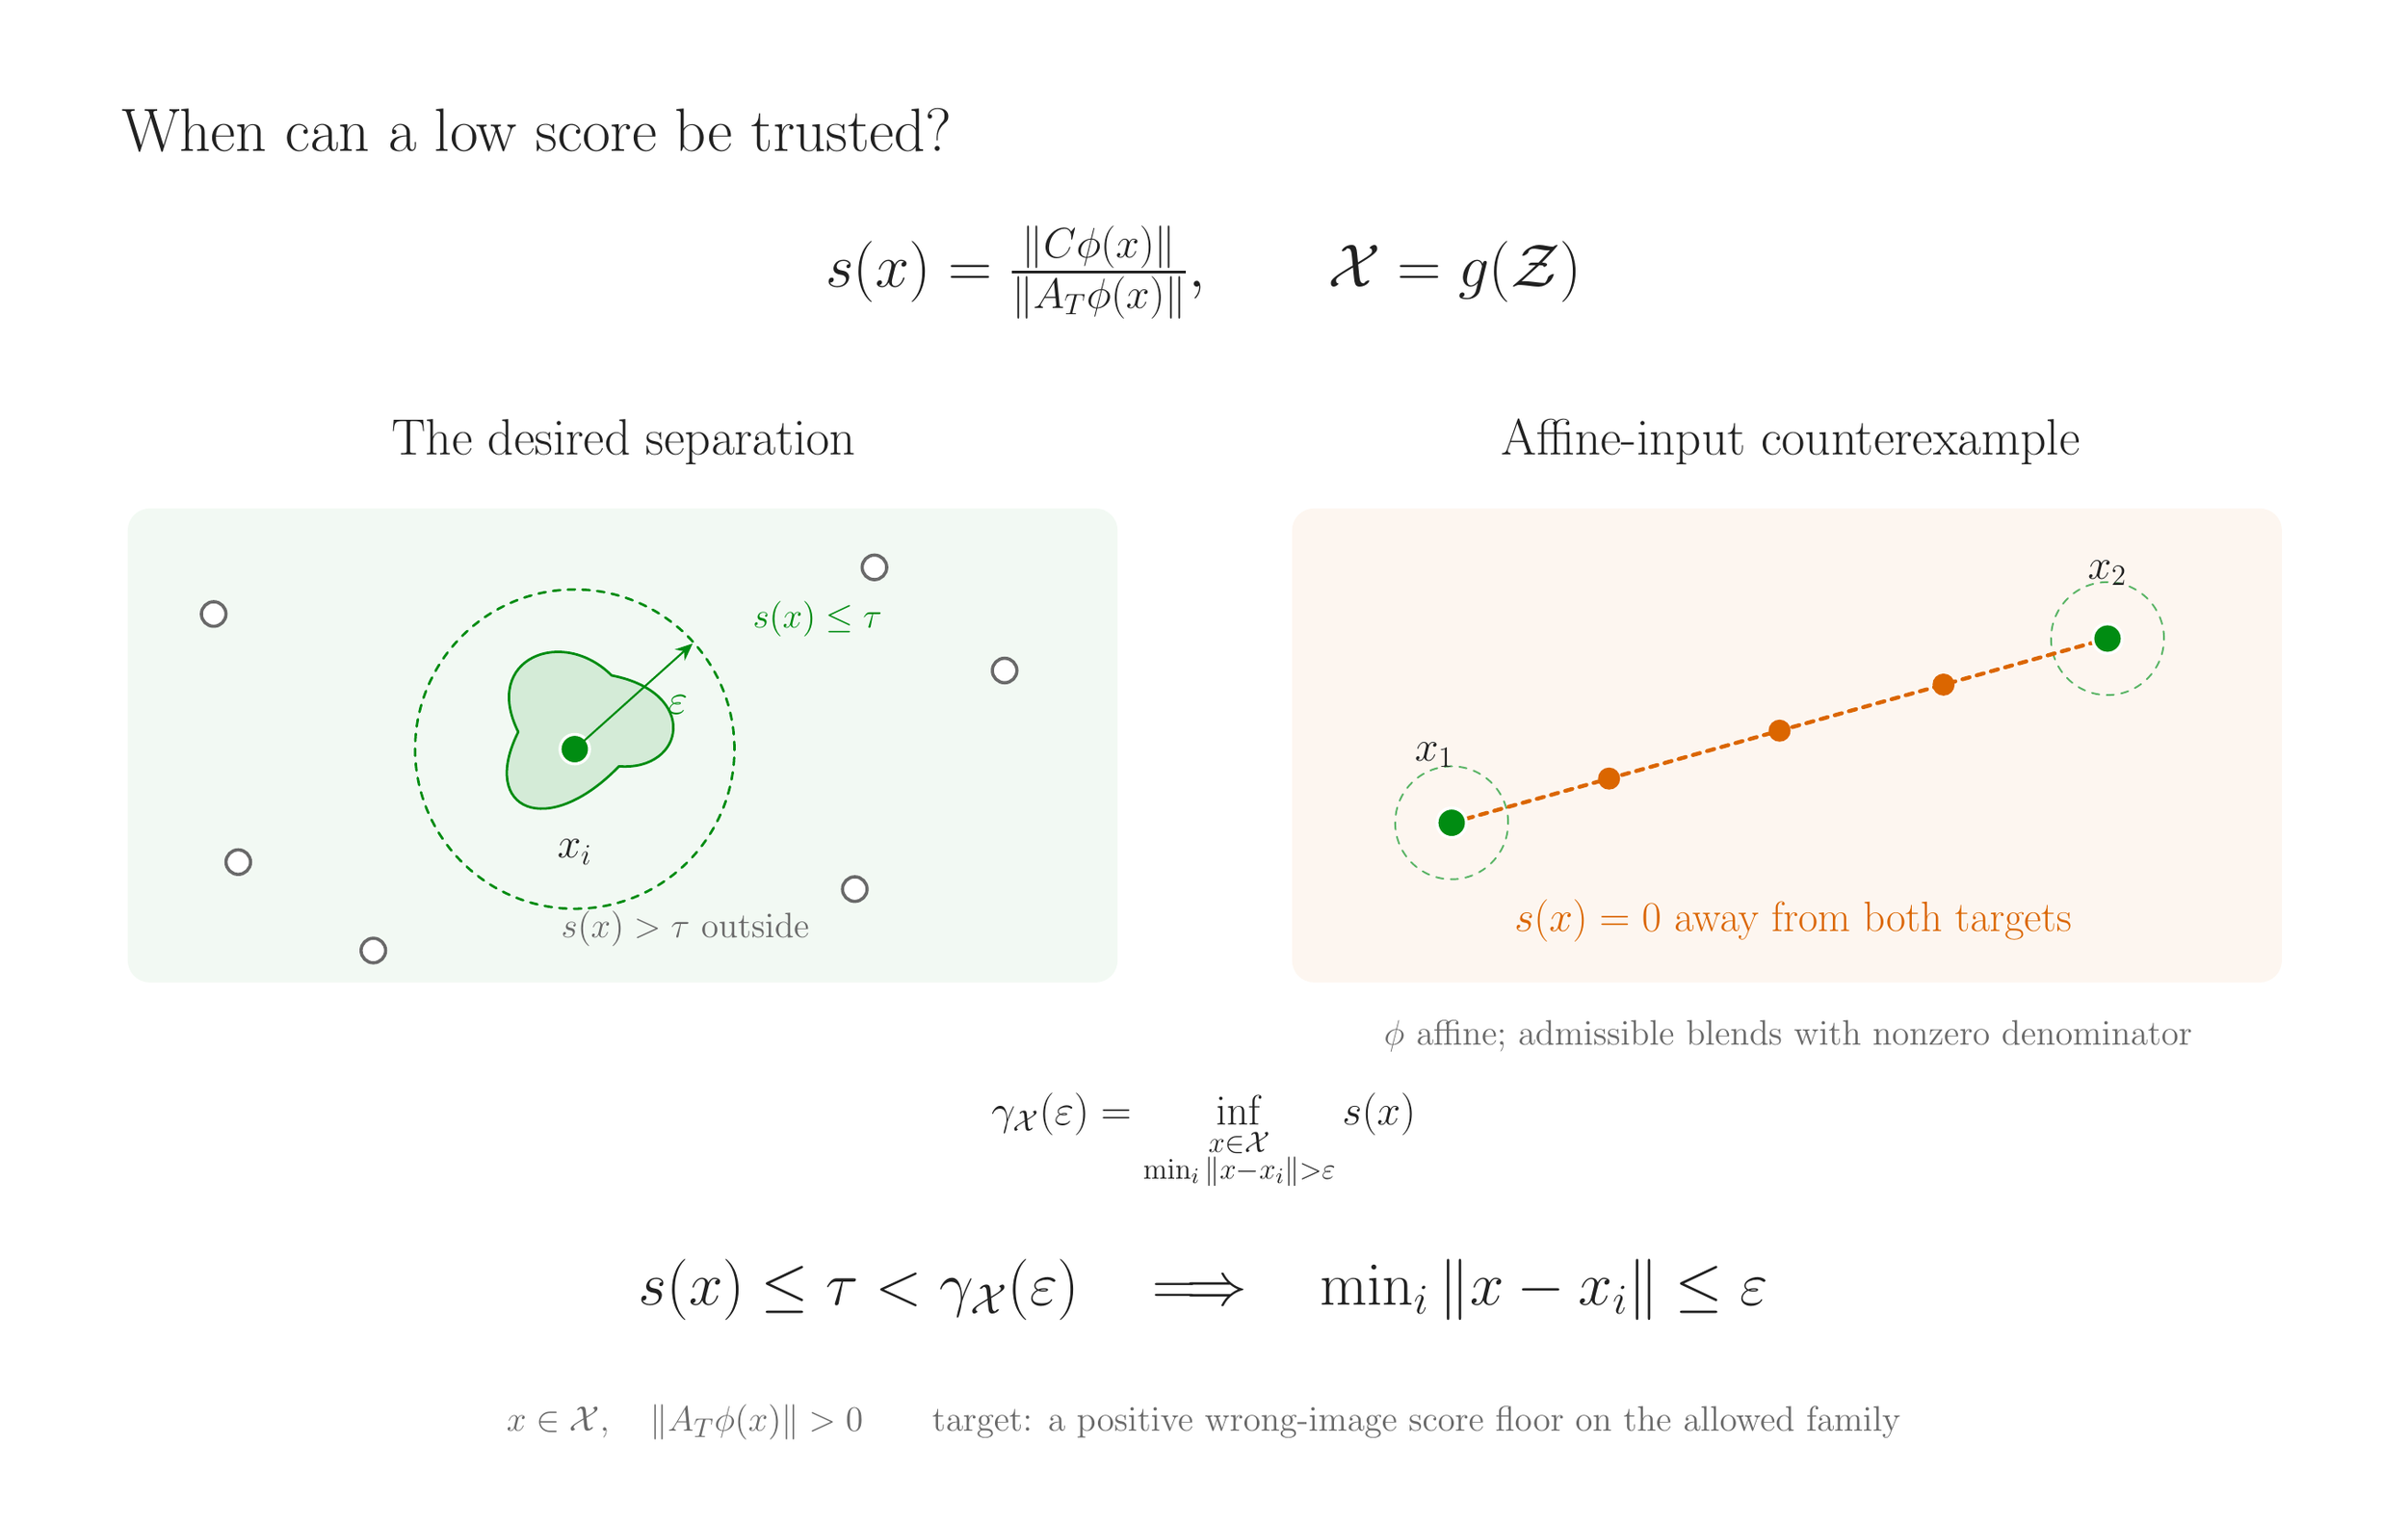
\begin{tikzpicture}[figure]
\canvas{When can a low score be trusted?}
\node[equation] at (480,499) {$s(x)=\frac{\|C\phi(x)\|}{\|A_T\phi(x)\|},\qquad
 \mathcal X=g(\mathcal Z)$};
\node[heading] at (244,430) {The desired separation};
\node[heading] at (719,430) {Affine-input counterexample};
\fill[family!5,rounded corners=9pt] (42,210) rectangle (445,403);
\fill[adapter!6,rounded corners=9pt] (516,210) rectangle (919,403);
\draw[draw=family,dashed,line width=1pt] (224,305) circle (65pt);
\path[draw=family,fill=family!17,line width=1pt]
 (201,312) .. controls (186,342) and (219,355) .. (239,335)
 .. controls (275,328) and (269,296) .. (242,298)
 .. controls (213,268) and (185,280) .. (201,312);
\node[target] at (224,305) {};
\node[labeltext] at (224,263) {$x_i$};
\draw[fineflow,draw=family] (224,305)--(272,348);
\node[labeltext,text=family] at (266,323) {$\varepsilon$};
\node[smalllabel,text=family,anchor=west] at (293,358) {$s(x)\le\tau$};
\foreach \x/\y in {77/360,87/259,346/379,399/337,338/248,142/223} \node[candidate] at (\x,\y) {};
\node[smalllabel,text=muted] at (269,232) {$s(x)>\tau$ outside};
\draw[dashed,draw=family!65,line width=.7pt] (581,275) circle (23pt);
\draw[dashed,draw=family!65,line width=.7pt] (848,350) circle (23pt);
\draw[dashed,adapter,line width=1.6pt] (581,275)--(848,350);
\foreach \a in {.24,.5,.75}{
 \fill[adapter] ({581+267*\a},{275+75*\a}) circle (4.5pt);
}
\node[target] at (581,275) {};
\node[target] at (848,350) {};
\node[labeltext,anchor=south] at (574,294) {$x_1$};
\node[labeltext,anchor=south] at (848,368) {$x_2$};
\node[labeltext,text=adapter] at (720,235) {$s(x)=0$ away from both targets};
\node[smalllabel,text=muted] at (718,188) {$\phi$ affine; admissible blends with nonzero denominator};
\node[labeltext] at (480,145) {$\displaystyle\gamma_{\mathcal X}(\varepsilon)=
 \inf_{\substack{x\in\mathcal X\\\min_i\|x-x_i\|>\varepsilon}}s(x)$};
\node[equation] at (480,85) {$s(x)\le\tau<\gamma_{\mathcal X}(\varepsilon)
 \quad\Longrightarrow\quad\min_i\|x-x_i\|\le\varepsilon$};
\node[smalllabel,text=muted] at (480,31) {$x\in\mathcal X,\quad\|A_T\phi(x)\|>0\qquad
 \text{target: a positive wrong-image score floor on the allowed family}$};
\end{tikzpicture}
\end{document}
